\chapter{Implementation of Spark based Semantic Document Matching}
\label{implementation}

In this chapter, we discuss the details involved in the implementation of the spark based Semantic Document Matching application. In \ref{section: implementation preferences}, we discuss in nutshell about the software and hardware preferences, dependency plug-ins and about the libraries from external sources that we used in our application. From \ref{section: loading data}, we discuss about how the implementations performed in detail and the example results for enhanced perspective.


\section{Implementation Preferences}
\label{section: implementation preferences}
In this section, we discuss the details of the implementation environment and the requirements which we used for our application development in various stages.

\subsection{Software Preferences}
We have used Python 3 as our programming language as it supports interactive shell, lambda expressions, and DataFrames. Though Python based implementation takes more time than Java and Scala based implementations with RDD APIs, it do not affect the performance of the DataFrame API. To carry out development on Ubuntu operating system, We used a virtual box environment called VMware and the following software are installed in the virtual environment:

\begin{itemize}
\item Python 3
\item PySpark 2.2
\item Jupyter notebook
\end{itemize}




\subsection{Plugin Preferences}
We have used Numpy and Scipy libraries \cite{website:numpy} for faster vector computations. To parse the extensible Markup Language (XML) file, we have used databricks XML data source library \cite{website:xmlspark}. It is an official API for the spark to read XML files by databricks. We also used Py4j library which connects the bridge between Python interpreter and the Java virtual machine \cite{website:py4j}. For parsing of XML documents in a non-parallel environment, a library available as python extension called minidom is used \cite{website:minidom}.


\section{Loading Data}
\label{section: loading data}
As illustrated in \ref{fig: Implementation_process}, the initial process of our application starts with the loading of data. The data we have chosen is in XML format and the glimpse of a single file can be seen in \ref{fig:reutersdoc}. Using databricks XML data source API and Spark SQL, the data is loaded into a DataFrame with a manually specified schema. For the process of document matching, we require each document id and associate paragraphs. Hence on performing SQL select operation on the input DataFrame, we get the \ref{fig: loadingdata1} as the initial DataFrame with two columns namely DocId and text where DocId is the identity of each document and text holds the paragraphs. Once the data is loaded into a DataFrame, with the use of show(), describe(), printSchema() methods the data can be analyzed. By default, the show method returns the first 20 rows of the DataFrame.
From \ref{fig: loadingdata1}, we can observe that the data in text column is raw which also contains special characters. Hence the next stage would be cleansing of the data. The code snippet for this stage is illustrated in \ref{lst:parsing and loading data}

\begin{lstlisting}[style=Java,float=htb,caption={Python code for parsing and loading of data into a DataFrame},label={lst:parsing and loading data}]
xmlDf = spark.read.format('com.databricks.spark.xml').\
	options(rowTag='newsitem').load('<fileDirectory>',schema= custom)
df_first= xmlDf.select(col("_itemid").alias("DocId"),'text')
\end{lstlisting}

\begin{figure}[tbp]
	\centering
		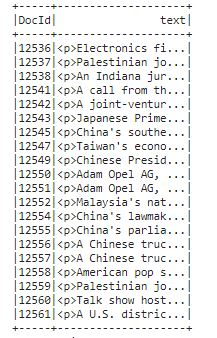
\includegraphics[scale=1.0]{loadingdata1}
	\caption{An output from loading data stage}
	\label{fig: loadingdata1}
\end{figure}

\section{Tokenization}
As discussed in the \ref{background}, the process of splitting a sentence or paragraph into individual words is referred as tokenization. ML package in Spark provides a powerful tokenizer API with which the process of the  tokenization can be performed. The tokenizer API is a transform function provided by the spark's ML library that transforms a DataFrame from one form to another form. The tokenizer API also supports the removal of special characters using regular expressions. Using regular expressions function, We have described the function to remove all the special characters, the numerical characters and convert all the words containing upper case to lower case. we have also described the minimum length of a character to be tokenized as 2 as a pre-requisite in order to retrieve the most meaningful words from the input dataset. The tokenizer API takes the text column as the input and returns an array of words in the new column. As shown in \ref{lst:tokenization}, with the tokenizer API, we can name the new column and we have named the new column as Words and is illustrated in \ref{fig: tokenization_output}. Using transform() operation, the tokenization is applied on the input DataFrame.

\begin{lstlisting}[style=Java,float=htb,caption={Python code for tokenization},label={lst:tokenization}]
tokens = RegexTokenizer(minTokenLength=2,inputCol='text',\
		 outputCol='Words', pattern="[^a-z]+") 
Tokenized = tokens.transform(df_first)
\end{lstlisting}

\begin{figure}[htbp]
	\centering
		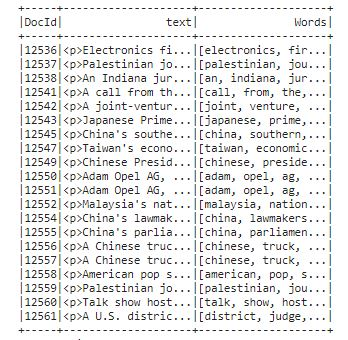
\includegraphics[scale=1.20]{tokenization_output}
	\caption{An output dataframe after tokenization stage }
	\label{fig: tokenization_output}
\end{figure}

\section{StopWords Removal}
As our input data is a huge collection of news articles, they often contain stop words in frequent. It is essential to clean those stop words in order to get meaningful terms. Spark's ML library provides the StopWords Remover function. It also comes under the transform function. The function takes an array of strings as input, applies the function and returns a new DataFrame with the addition of output column. The output DataFrame from this step is illustrated in \ref{fig: stopwords_output}.  The function is applied using transform() operation on the output DataFrame from the tokenization stage. The code snippet for this stage is shown in \ref{lst:stopwords}.

\begin{lstlisting}[style=Java,float=htb,caption={Python code for removal of stop words},label={lst:stopwords}]
Tokens_filtered = StopWordsRemover(inputCol='Words',\
				  outputCol='filtered_words')
Tokenized_filtered = Tokens_filtered.transform(Tokenized)
\end{lstlisting}

\begin{figure}[htbp]
	\centering
		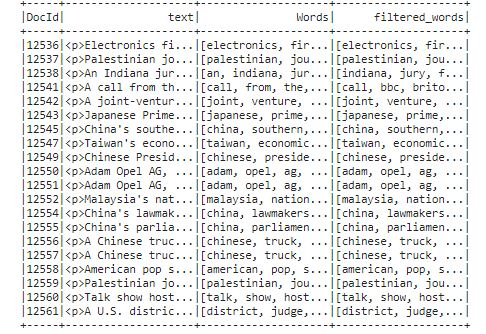
\includegraphics[scale=1.20]{stopwords_output}
	\caption{An output dataframe after cleaning of stop words }
	\label{fig: stopwords_output}
\end{figure}

\section{Count Vectorizer}
As discussed earlier in \ref{section: countvectorizer}, with the help of count vectorizer, any document can be converted to a sparse vector representation. Spark provides this functionality under the hood of extractors in the ML package. In order to convert a document into a sparse vectors, the function requires fit() and transform() operations as shown in \ref{lst:count vectorizer}. Firstly, on applying fit() operation the count Vectorizer builds a model by mapping the unique words to unique IDs that are extracted from the filtered words column. When transform() operation is applied, the count vectorizer transforms the documents representing an array of words to a sparse vector with the help of a dictionary. From \ref{fig: cv_output}, we can observe the DataFrame containing various stage of transformations of a document starting from loading of raw data to sparse vector representation of a document. 

\begin{lstlisting}[style=Java,float=htb,caption={Python code to perform count vectorization},label={lst:count vectorizer}]
cv = CountVectorizer(inputCol="filtered_words", outputCol="features")
cv_model = cv.fit(Tokenized_filtered)     
result = cv_model.transform(Tokenized_filtered)
result1 = result.select('DocId','features')
\end{lstlisting}

\par As discussed earlier about the vector representation of a document, we can observe from the features column in \ref{fig: cv_output} for a given example input, the total number of unique terms found by the count vectorizer model is 9844 which can also be referred as vocabulary size.

\begin{figure}[htbp]
	\centering
		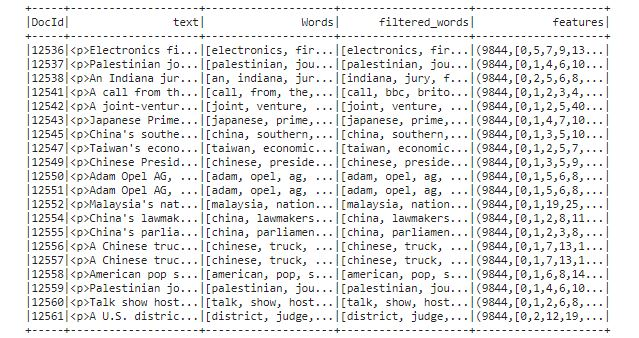
\includegraphics[scale=0.90]{cv_output}
	\caption{An output dataframe after performing count vectorization on input words }
	\label{fig: cv_output}
\end{figure}


\begin{figure}[htbp]
	\centering
		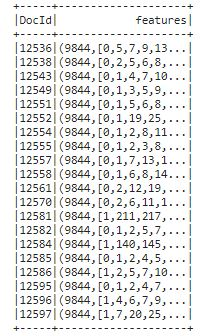
\includegraphics[scale=1.00]{cv1_output}
	\caption{An output dataframe after performing SQL Query }
	\label{fig: cv1_output}
\end{figure}

\par Additionally, the count Vectorizer model provides various parameters for tuning the model while creation. By default, the count vectorizer function selects the terms whose frequency of appearance is at least two times. But, we have set the value to 1 as we need each and every word that constituting to the document. On performing Spark SQL select operations on the DataFrame as in \ref{fig: cv_output}, we have only taken two columns and can be seen in \ref{fig: cv1_output} since the next stage only relays on feature column and DocId column. By reducing the DataFrame size, we can reduce the load on in-memory computations there by increasing the performance of the application.  


\section{Latent Dirichlet Allocation}
Recollecting from \ref{section: lda}, LDA approach is used for two reasons. The prime reason is to represent the document in terms of topic distribution and the other is to reduce the dimensionality of the vector representation achieved from the previous stage.

\begin{lstlisting}[style=Java,float=htb,caption={Python code to perform LDA Topic Modeling },label={lst:LDA}]
lda = LDA(k=90,maxIter=20,optimizer = "em")       
model = lda.fit(result1)
lda_df = model.transform(result1)
\end{lstlisting}


\par We have used LDA API under the Spark's ML package. From the \ref{lst:LDA}, the number of topics (k) that a document to be presented has to be manually specified. Hence, we have set the topics(K) to 90. Similarly, the number of iterations also has to be manually specified. The iterations represent the times an Estimation-Maximization (EM) algorithm has to infer the topics. At first iteration, the EM algorithm randomly assigns the words to every topic. From the second iteration, the M-step updates the parameters by learning the latent topics discovered from the previous iteration and the word assignment to topics based on the present parameters is performed again at each iteration. Since our focus was not to calculate the convergence but the runtime, we have set the iterations to 20. LDA also requires fit() and transform() operations to build the topic distribution. 

\begin{figure}[htbp]
	\centering
		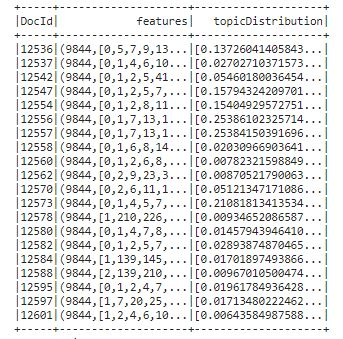
\includegraphics[scale=1.20]{lda_output}
	\caption{An output dataframe consisting of topic distribution after LDA modeling on the input dataset }
	\label{fig: lda_output}
\end{figure}

\par When fit() operation is applied on DataFrame from the previous stage as in \ref{fig: cv1_output}, LDA starts constructing the document topic matrix from a sparse vector. At this state, the entire input dataset is divided to all worker nodes in a cluster. The worker nodes construct topic distributions locally with the available data and send back to the driver using broadcast variables resulting in a huge combined matrix. Now, when the  transform() operation is applied, the DataFrame transforms to the other consisting of an additional column named topicDistribution. The output DataFrame is illustrated in \ref{fig: lda_output}. As we set the number of topics to 90, every document is represented by a vector of 90 dimensions and are in dense vector representation.  Since the LDA representation of the document is a probabilistic distribution, the summation of all topic values results to 1 for every document.


\section{Document Pair Comparison}
\label{implement: Document Pair Comparison}
In this stage, we perform a comparison of each document to every other document in the entire corpus. Using the Spark SQL, a self-join is performed on the Same DataFrame from the previous stage by aliasing the column names and is illustrated in \ref{fig: comparison}. Hence, this stage in the Document matching process consumes most of the time for performing the computations as the process requires a total of  \(O(n^2)\) computations.

\begin{figure}[htbp]
	\centering
		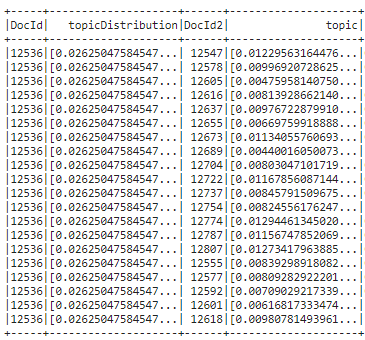
\includegraphics[scale=1.20]{comparison}
	\caption{An output dataframe after performing self join operation }
	\label{fig: comparison}
\end{figure}



For example, let us consider three documents namely Document 1, Document 2, and Document 3 present in a DataFrame. A total of 6 combinations results when a self-join is applied on the DataFrame and is illustrated in \ref{tab:combinations}. 


\begin{table}[htbp]
	\centering
		\begin{tabular}{cc}\toprule
		DocId	& DocId2\\\midrule
		1 & 2\\\addlinespace 
		1 & 3\\\addlinespace
		2 & 1\\\addlinespace
        2 & 3\\\addlinespace
        3 & 1\\\addlinespace
		3 & 2 \\\bottomrule
		\end{tabular}
	\caption{An example of document combinations}
	\label{tab:combinations}
\end{table}

\begin{equation}\label{formula: hellinger on two documents}
Hellinger(1,2) == Hellinger(2,1)
\end{equation}

But from \ref{formula: hellinger on two documents}, we can observe that the Hellinger metric assures from the symmetric property which translates to the result obtained by the product of any two documents are same irrespective of the order they appear. Hence, we have passed the \ref{formula: pair condition} as join condition in order to decrease the number of computations required in calculating the total document pairs. By passing this condition, we can eliminate computations of the document pairs that are symmetric to already computed pairs. For example, by applying \ref{formula: pair condition} the total computations in \ref{tab:combinations} can be reduced to 3 which translates to speed up of the computation process by a percentage of 50. The code listing is illustrated in \ref{lst:pairwise}.

\begin{equation}\label{formula: pair condition}
DocId < DocId2
\end{equation}

\begin{lstlisting}[style=Java,float=htb,caption={Python code to perform Document Pair Comparison },label={lst:pairwise}]
similarity_df = final_df.join(final_df.alias("copy_df").\
     	select(col("DocId").alias("DocId2"),col("topicDistribution").\
     	alias("topic")),col("DocId") < col("DocId2"), 'inner')
		.withColumn('Score',hellinger_udf(col('topicDistribution'),\
		col('topic')))
\end{lstlisting}


\par Using withColumn() operation, a new column named Score is added to the DataFrame as in \ref{fig: comparison1}. The result of calculating the distance between topic distribution of two documents is stored in the Score column. The score value represents the similarity between the two documents. The distance is calculated using Hellinger distance metric as already discussed in \ref{section: document pair comparison}. As Spark do not have the built-in Hellinger function, we have created a user defined function using Spark's udf() functionality.  

\begin{figure}[htbp]
	\centering
		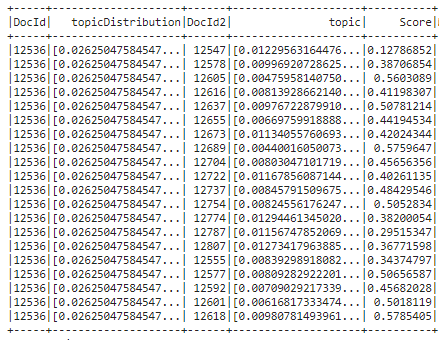
\includegraphics[scale=1.20]{comparison1}
	\caption{An output dataframe from Document Pair Comparison Stage }
	\label{fig: comparison1}
\end{figure}


\section{Classification}

In this stage, every document pair is classified as either match or non-match based on their obtained similarity score. A user defined function holding a threshold condition is manually specified to classify the document pairs using udf(). The condition for classification is shown in \ref{formula: threshold condition} and \ref{formula: threshold condition1} respectively where 1 represents that the two documents are semantically similar and 0 represents the documents are dissimilar.

\begin{equation}\label{formula: threshold condition}
\textit{Score}   >  \textit{threshold-value}  \Rightarrow Match = 0
\end{equation}
\begin{equation}\label{formula: threshold condition1}
\textit{Score}  \leq  \textit{threshold-value}  \Rightarrow Match = 1
\end{equation}


\par As shown in \ref{lst:classification}, using withColumn() a new column  named Match\char`_result is appended to the DataFrame from previous stage as shown in \ref{fig: classification}. The threshold function is performed on the column score and the obtained result is stored in the column Match\char`_result.

\begin{lstlisting}[style=Java,float=htb,caption={Python code to classify Documents along with threshold condition},label={lst:classification}]
def threshold(Score):
    if Score <= 0.2:
        return 1
    else:
        return 0
        
output_df = similarity_df.withColumn('Match_result',\
			threshold_udf(col('Score'))
\end{lstlisting}

\begin{figure}[htbp]
	\centering
		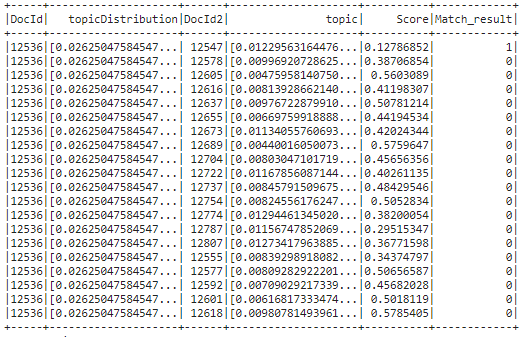
\includegraphics[scale=1.00]{Classification}
	\caption{An output dataframe from Classification stage }
	\label{fig: classification}
\end{figure}

\section{Evaluation}
\label{implement:evaluation}

The final stage in our implementation process is Evaluation. With the results obtained from the classification stage, evaluations are computed to calculate the speed-up, efficiency and effectiveness and are discussed in detail in \ref{evaluation}. 

\par To calculate the effectiveness of an implementation, the results obtained from our process need to be matched with the golden data. But as discussed in \ref{section: rcv1}, the corpus do not possess any ground truth information representing the similarity state of two documents but provides information of a document belongs to a topic. Hence we have implemented a workaround method to extract the topics from the metadata information available from each document. The glimpse of a document is presented in \ref{fig:reutersdoc}. The workaround method is implemented as a combination of parallel and a non-parallel environment i.e. with the combination of Python and Spark framework. The steps involved in workaround method is discussed below:


\subsection{Parsing XML}
\par Using minidom \cite{website:minidom} which is a Python extension library, each document is parsed to extract the topic information available under the metadata information. The data obtained is stored as a list of lists and is illustrated in \ref{lst:minidom}. Each list contains information of the document ID and list of topics, as a document can speak about different topics. Due to the complex structure of the input document, the extracted category information is obtained as a combination of regions and topics. Hence to increase the accuracy of the data, it is necessary to remove the regions from the topics.

\begin{lstlisting}[style=Java,float=htb,caption={Python Code to parse XML file to extract category using minidom library in non-parallel Environment},label={lst:minidom}]
from xml.dom import minidom
import os
directory = '<fileDirectory>'
finallist = []

for root,dirs,filenames in os.walk(directory):
        for file in filenames:
            #print(file)
            log = open(os.path.join(root,file),'r')
            doc = minidom.parse(os.path.join(root,file))
            idlist = doc.getElementsByTagName('newsitem')
            for id in idlist:
                value = id.getAttribute("itemid")
            codelist = doc.getElementsByTagName('code')
            words=[]
            for s in codelist:
                words.append(s.attributes['code'].value)
            finallist.append(value)
            finallist.append(words)

\end{lstlisting}

\newpage
\subsection{Removal of Regions}
\par As discussed in the earlier chapter, Spark provides many powerful tools for the purpose of pre-processing. One among them is stop words remover. To use the Spark's component, firstly the data is loaded into a DataFrame using a manually specified schema with createDataFrame() operation. Using the Reuters data file, a list consisting of all the region codes is generated as a stop words list . Using the stop words list, all the regions are removed and the DataFrame transformation is performed using transform(). The code for this step can be observed in \ref{lst:extract regions}.

\begin{lstlisting}[style=Java,float=htb,caption={Python Code for loading lists into DataFrame and filter regions},label={lst:extract regions}]
df_first = spark.createDataFrame([(x,y) for x,(y) in (zip(
            islice(finallist,0,len(finallist),2),
           islice(finallist,1,len(finallist),2)))],\
           ('DocID','Categories'))
Filter_regions = StopWordsRemover(inputCol='Categories',\
				 outputCol='Topics',stopWords=["list"])
\end{lstlisting}



\subsection{Pair Comparison} 

\begin{table}[htbp]
	\centering
		\begin{tabular}{cc}\toprule
		DocId	& Topics\\\midrule
		1 & Apple, Bat\\\addlinespace 
		2 & Bat, Cat, Dog\\\addlinespace
		3 & Apple \\\bottomrule
		\end{tabular}
	\caption{An example of document and topics}
	\label{tab:document topics}
\end{table}

This step is similar to the stage in the document matching process. In this step, we performed the comparison of each document with every other document. A self-join of the same DataFrame by aliasing the column names is performed. The similar join condition as in \ref{formula: pair condition} used in document pair comparison is used here also in order to obtain the exact document pairs. Using withColumn(), a new column is appended to the DataFrame named Intersect\char`_score. The score is generated as a true or false and is stored in the Intersect\char`_score column. Two documents are said to be true if any of the topics overlap between the two documents. It is false if there is no overlap in between two document topics. For example, let us consider three documents and the 4 topics. Each document is provided with topics that a document belongs to and is illustrated in \ref{tab:document topics}.


\begin{equation}\label{formula: pair condition for subset}
Topics(DocId) \subset Topics(DocId2) \Rightarrow True
\end{equation}
\begin{equation}\label{formula: pair condition for not subset}
Topics(DocId) \not\subset Topics(DocId2) \Rightarrow False
\end{equation}


Based on the \ref{formula: pair condition for subset} and \ref{formula: pair condition for not subset}, the \ref{tab:score generation} is generated.


\begin{table}[htbp]
	\centering
		\begin{tabular}{ccc}\toprule
		DocId	& DocId2 & Score\\\midrule
		1 & 2 & True\\\addlinespace 
		1 &  3 & True\\\addlinespace
        2 & 3 & False\\\bottomrule
		\end{tabular}
	\caption{A Table illustrating Score generation}
	\label{tab:score generation}
\end{table}

\subsection{Classification} 
Based on the Score obtained from the previous step, every document pair is classified as similar or dissimilar according to the \ref{formula: threshold condition for category} and \ref{formula: threshold condition1 for category} where 1 represents that a document pair contains the common topics between them and 0 represents that a document pair do not hold any common topics between them. A new column is appended to the previous stage DataFrame using withColumn() and the classification results obtained in this step are stored in this column.

\begin{equation}\label{formula: threshold condition for category}
\textit{Score}   \equiv  \textit{True}  \Rightarrow True\char`_match = 1
\end{equation}
\begin{equation}\label{formula: threshold condition1 for category}
\textit{Score}  \equiv  \textit{False}  \Rightarrow True\char`_match = 0
\end{equation}


\begin{figure}[htbp]
	\centering
		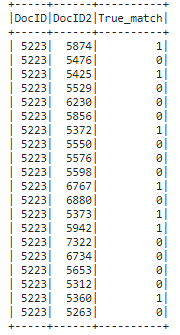
\includegraphics[scale=1.05]{category_extraction}
	\caption{An output dataframe obtained in the Category Extraction Process }
	\label{fig: category_extraction}
\end{figure}

\begin{lstlisting}[style=Java,float=htb,caption={Python Code for writing resulting DataFrame to parquet Format},label={lst:write parquet}]
Final.write.parquet('<FileLocation>')
\end{lstlisting}

\newpage
Finally as shown in \ref{lst:write parquet}, the resulting DataFrame obtained is written to the parquet file and is stored. The final DataFrame obtained after processing all the steps is shown in \ref{fig: category_extraction}. The DataFrame obtained from classification stage is compared to the DataFrame obtained in this process. By applying Spark DataFrame count() method on the resulting DataFrame, the number of True Positives, False Negatives, False Positives, and True Negatives are calculated with which measures like recall, precision and F-measure are calculated.







%In diesem Kapitel beschreiben Sie,
%- wie Sie versucht haben, Ihre Arbeit (z.B. Programm, Theorie, oder Algorithmus) zu verifizieren
%- Hierfür haben Sie bereits im Kapitel 3 Prognosen oder Qualitätskriterien aufgestellt, die Sie hier überprüfen
%Zu jeder zu überprüfenden Eigenschaft sollten Sie
%- ein geeignetes Experiment entwerfen, um diese Eigenschaft zu überprüfen
%- dieses Experiment beschreiben und durchführen
%- die Ergebnisse geeignet präsentieren und kommentieren

%wie lange dauert das schlussfolgern bei bestimmten veränderungen?
%wie lange für komplett unterschiedliche?


